\documentclass[12pt,a4paper]{article}
\usepackage[margin=1in]{geometry}
\usepackage[T1]{fontenc}
\usepackage{lmodern}
\usepackage{microtype}
\usepackage{amsmath,amssymb}
\usepackage{booktabs,array,tabularx}
\usepackage{graphicx}
\usepackage{xcolor}
\usepackage{tikz}
\usetikzlibrary{arrows.meta,positioning,fit}
\usepackage{caption}
\usepackage{hyperref}
\usepackage{xurl}
\hypersetup{colorlinks=true,linkcolor=black,urlcolor=blue!55!black}
\urlstyle{tt}
\setlength{\parindent}{0pt}
\setlength{\parskip}{4pt}
\setlength{\emergencystretch}{3em}
\setlength{\abovecaptionskip}{5pt}
\setlength{\belowcaptionskip}{2pt}
\captionsetup{font=small,labelfont=bf}
\definecolor{naf}{HTML}{F4A261}
\definecolor{cond}{HTML}{8ECAE6}
\definecolor{wav}{HTML}{90BE6D}
\definecolor{ink}{HTML}{23313D}
\color{ink}
\newcommand{\codepath}[1]{\begingroup\small\ttfamily\raggedright\path{#1}\par\endgroup}

\begin{document}

\begin{center}
{\LARGE\bfseries Noise-Conditioned Wavelet NAFNet for Blind\\[3pt] Low-Light sRGB Denoising\par}
\vspace{0.55em}
{\large Team Voxel}\par
\vspace{0.35em}
{\normalsize Mora SP Cup 2026 --- Final Model Report}\par
{\small One-hour DirectML fine-tuning experiment; checkpoint selected by validation composite}
\end{center}

\section{Problem and scoring objective}
The task is blind denoising of $992\times992$ 8-bit sRGB low-light photographs. Corruption strength varies by image, and no noise-level metadata is available at inference. The official score is computed per image and then averaged:
\begin{equation}
\mathrm{composite}=0.6\,\mathrm{clip}\!\left(\frac{\Delta\mathrm{PSNR}}{15},0,1\right)
+0.4\,\max(\Delta\mathrm{SSIM},0),
\end{equation}
where each delta is the improvement over the original noisy image. The $0.6/15=0.04$ gain per dB makes the metric PSNR-led, while SSIM rewards structure preservation. The model therefore predicts a residual at the original exposure; it performs no gamma correction, tone mapping, or global brightness adjustment.

This report documents the final NCW-NAFNet experiment: the protected NAFNet baseline is wrapped with analytical noise conditioning, a learned noise refiner, an impulse feature, and fixed Haar-detail injections. The baseline checkpoint is never modified. All added paths start at exact identity through zero scalar gates.

\section{Measured degradation model}
The same 460 public noisy/clean pairs used in the attached Voxel report establish the design assumptions. Residual variance is heteroscedastic, $\operatorname{var}(I)=aI+b$, with normalized per-channel coefficients
\[
a=(0.017095,0.016532,0.019045),\qquad
b=(0.006362,0.005684,0.005492).
\]
The read-noise floor dominates dark regions, severity forms a continuum, and the residual is heavy-tailed with sparse impulses. These observations motivate spatial, content-dependent conditioning rather than a single global noise level. They also motivate wavelet details, which expose high-frequency corruption without changing the RGB input itself.

\clearpage
\section{Final architecture}
\textbf{Restoration backbone.} The backbone is NAFNet (width 32), with encoder depths $[2,2,4,8]$, 12 middle blocks, decoder depths $[2,2,2,2]$, and channel widths $32,64,128,256,512$. Each NAFBlock uses LayerNorm, pointwise expansion, depthwise $3\times3$ convolution, SimpleGate, simplified channel attention, and two learned residual scales. PixelShuffle performs decoder upsampling. The network predicts a residual that is added to the padded input.

\begin{figure}[h]
\centering
\resizebox{\textwidth}{!}{%
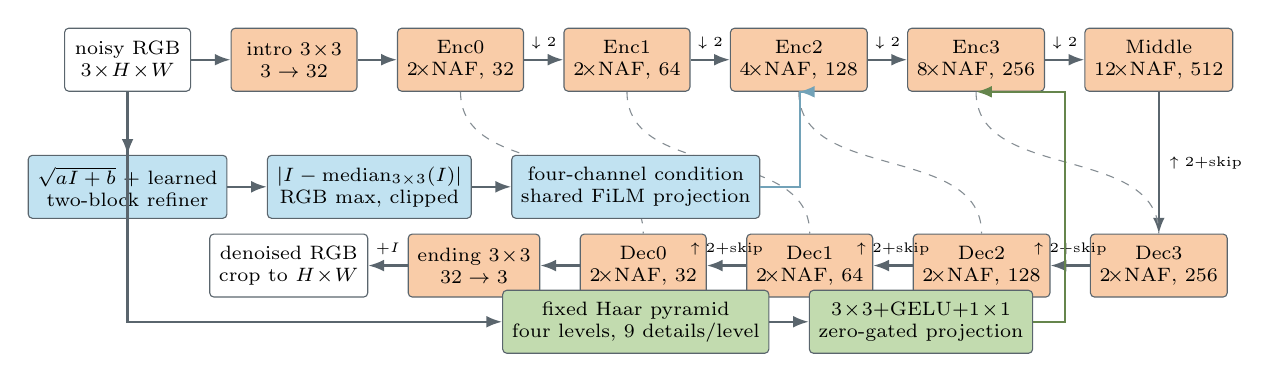
\begin{tikzpicture}[
  node distance=4.5mm and 5mm,
  box/.style={draw=ink!75,rounded corners=1.5pt,minimum height=8mm,minimum width=16mm,align=center,font=\scriptsize},
  core/.style={box,fill=naf!55},
  cb/.style={box,fill=cond!55},
  wb/.style={box,fill=wav!55},
  arr/.style={-{Latex[length=2mm]},thick,draw=ink!75}
]
\node[box] (in) {noisy RGB\\$3\!\times\!H\!\times\!W$};
\node[core,right=of in] (intro) {intro $3\!\times\!3$\\$3\to32$};
\node[core,right=of intro] (e0) {Enc0\\$2\!\times$NAF, 32};
\node[core,right=of e0] (e1) {Enc1\\$2\!\times$NAF, 64};
\node[core,right=of e1] (e2) {Enc2\\$4\!\times$NAF, 128};
\node[core,right=of e2] (e3) {Enc3\\$8\!\times$NAF, 256};
\node[core,right=of e3] (mid) {Middle\\$12\!\times$NAF, 512};
\draw[arr] (in)--(intro); \draw[arr] (intro)--(e0); \draw[arr] (e0)--node[above,font=\tiny]{$\downarrow2$}(e1);
\draw[arr] (e1)--node[above,font=\tiny]{$\downarrow2$}(e2); \draw[arr] (e2)--node[above,font=\tiny]{$\downarrow2$}(e3);
\draw[arr] (e3)--node[above,font=\tiny]{$\downarrow2$}(mid);

\node[core,below=18mm of mid] (d3) {Dec3\\$2\!\times$NAF, 256};
\node[core,left=of d3] (d2) {Dec2\\$2\!\times$NAF, 128};
\node[core,left=of d2] (d1) {Dec1\\$2\!\times$NAF, 64};
\node[core,left=of d1] (d0) {Dec0\\$2\!\times$NAF, 32};
\node[core,left=of d0] (end) {ending $3\!\times\!3$\\$32\to3$};
\node[box,left=of end] (out) {denoised RGB\\crop to $H\!\times\!W$};
\draw[arr] (mid)--node[right,font=\tiny]{$\uparrow2+$skip}(d3); \draw[arr] (d3)--node[above,font=\tiny]{$\uparrow2+$skip}(d2);
\draw[arr] (d2)--node[above,font=\tiny]{$\uparrow2+$skip}(d1); \draw[arr] (d1)--node[above,font=\tiny]{$\uparrow2+$skip}(d0);
\draw[arr] (d0)--(end); \draw[arr] (end)--node[above,font=\tiny]{$+I$}(out);
\draw[dashed,draw=ink!55] (e0.south) to[out=-90,in=90] (d0.north);
\draw[dashed,draw=ink!55] (e1.south) to[out=-90,in=90] (d1.north);
\draw[dashed,draw=ink!55] (e2.south) to[out=-90,in=90] (d2.north);
\draw[dashed,draw=ink!55] (e3.south) to[out=-90,in=90] (d3.north);

\node[cb,below=8mm of in] (ana) {$\sqrt{aI+b}$ + learned\\two-block refiner};
\node[cb,right=of ana] (imp) {$|I-\mathrm{median}_{3\times3}(I)|$\\RGB max, clipped};
\node[cb,right=of imp] (film) {four-channel condition\\shared FiLM projection};
\draw[arr] (in)--(ana); \draw[arr] (ana)--(imp); \draw[arr] (imp)--(film);
\draw[arr,draw=cond!80!black] (film.east) -- ++(5mm,0) |- (e2.south);

\node[wb,below=9mm of film] (haar) {fixed Haar pyramid\\four levels, 9 details/level};
\node[wb,right=of haar] (adapt) {$3\!\times\!3+$GELU$+1\!\times\!1$\\zero-gated projection};
\draw[arr] (in.south) |- (haar.west); \draw[arr] (haar)--(adapt);
\draw[arr,draw=wav!70!black] (adapt.east) -- ++(4mm,0) |- (e3.south);
\end{tikzpicture}
}
\caption{Complete NCW-NAFNet graph. The pretrained NAFNet core is orange, noise conditioning is blue, and fixed-Haar detail injection is green. Dashed lines denote encoder--decoder skips.}
\end{figure}

\textbf{Noise conditioning.} The analytical branch computes $\sqrt{aI+b}$ in normalized intensity units. A small 16-channel, two-NAFBlock refiner predicts a bounded correction. In parallel, an exact $3\times3$ median implemented as a min/max sorting network produces a robust one-channel impulse feature. Concatenation gives four channels. At every encoder stage and at the middle, a shared $3\times3$ projection and two $1\times1$ heads generate FiLM fields:
\[
F'=(1+g_\gamma\tanh\gamma(C))\odot F+g_\beta\beta(C).
\]
Both scalar gates are initialized to zero.

\textbf{Wavelet conditioning.} A differentiable four-level orthonormal Haar transform recursively decomposes the LL band. At each scale, RGB LH, HL and HH details form nine channels. A $3\times3\to\mathrm{GELU}\to1\times1$ adapter projects them to the matching feature width and adds them after downsampling through a zero-initialized scalar gate. The full model has 29,664,484 parameters: 29,159,715 in the untouched backbone and 504,769 in the added conditioning and wavelet modules.

\section{Identity safety and implementation checks}
The pretrained checkpoint is loaded with a strict tensor match: all 664 backbone tensors must load, with no missing, unexpected, or shape-mismatched key. With every new scalar gate at zero, the wrapper output is numerically identical to the backbone; the preflight test measured maximum absolute difference 0.0 on the DirectML device.

Protected baseline SHA-256:
\codepath{6acdff27227bbde63386f37fb07f06d3db08656bb76b38ae3f3f2c240c903ae8}

Two platform-specific repairs were required. First, PyTorch's AdamW uses an in-place \texttt{lerp\_} update unsupported by the installed DirectML backend. A mathematically equivalent AdamW implementation based on \texttt{mul\_}, \texttt{add\_}, \texttt{addcmul\_}, and \texttt{addcdiv\_} removed that path. Second, whole-image NCW validation triggered a native \texttt{c10.dll} access violation. Validation now stages $256\times256$ overlap tiles from CPU, processes bounded DirectML crops with a 64-pixel halo, and performs raised-cosine accumulation on CPU. The official evaluator still scores complete, quantized $992\times992$ predictions.

\section{One-hour training protocol}
The model was trained in float32 on DirectML with batch size 1 and random $256\times256$ patches. Each sample was a real noisy/clean pair with probability 0.70; otherwise the clean patch was corrupted by the fitted generalized noise synthesizer. The objective was
\[
L=0.90L_{\mathrm{PSNR}}+0.10L_{\mathrm{SSIM}},
\]
with gradient norm clipped at 1.0. The optimizer used $\beta=(0.9,0.9)$ and weight decay $10^{-3}$.

\begin{table}[h]
\centering\small
\begin{tabularx}{\textwidth}{@{}>{\raggedright\arraybackslash}p{0.18\textwidth}>{\raggedright\arraybackslash}p{0.16\textwidth}>{\raggedright\arraybackslash}X>{\raggedright\arraybackslash}p{0.25\textwidth}@{}}
\toprule
Phase & Interval & Trainable parameters & Backbone / adapter LR \\
\midrule
A: adapter activation & steps 0--999 & NCW additions only & $0\,/\,3.0\times10^{-4}$ \\
B: targeted tuning & steps 1000--3424 & middle, decoder, output + NCW & $3.0\times10^{-5}\,/\,1.5\times10^{-4}$ \\
C: low-LR refinement & 40--52 min & full model & cosine from $1.2\times10^{-5}\,/\,7.0\times10^{-5}$ \\
\bottomrule
\end{tabularx}
\caption{Three training phases. Phase C began at step 3425 and decayed to $1.8\times10^{-6}/1.05\times10^{-5}$ at the optimizer cutoff.}
\end{table}

Optimization stopped at 52 minutes to reserve time for full validation, checkpoint selection, reload, and final verification. The run completed 4,122 optimizer steps and five validation epochs in 58.3 minutes. A validation epoch means 1,000 optimizer steps followed by all 46 held-out images; epoch 5 is the final partial interval.

\section{Validation methodology}
The 460 public pairs use the same deterministic severity-stratified split as the attached Voxel report: 414 images for training and 46 for validation. Image IDs 461--480 are excluded from all fitting, checkpoint selection, and metric computation. Every validation prediction is clipped, rounded as $\lfloor255x+0.5\rfloor$, saved as PNG, and scored by the unmodified \texttt{evaluation/evaluate.py}. Thus PSNR, SSIM and the composite below include the exact 8-bit quantization used for test outputs.

The baseline comparison is the protected report value evaluated by whole-image inference, whereas the NCW measurements use the required tiled DirectML path. The numbers are official for their respective outputs, but the inference geometry is not perfectly matched. The conclusion is still unambiguous because the NCW deficit is much larger than its epoch-to-epoch variation.

\section{Results}
The final best-composite model achieves \textbf{31.3046 dB PSNR}, \textbf{0.919337 SSIM}, and \textbf{0.63462481 composite}. Relative to the protected baseline, this is $-0.3254$ dB, $-0.000163$ SSIM, and $-0.008675$ composite ($-1.35\%$). The requested 33 dB target was not achieved; the remaining gap is 1.6954 dB.

\begin{table}[h]
\centering\small
\resizebox{\textwidth}{!}{%
\begin{tabular}{@{}r r c r r r r@{}}
\toprule
Epoch & Step & Phase & PSNR & SSIM & Composite & $\Delta$ composite vs. baseline \\
\midrule
1 & 1000 & A & 31.3039 & 0.919125 & 0.634218 & $-0.009082$ \\
2 & 2000 & B & 31.2968 & 0.918920 & 0.634052 & $-0.009248$ \\
3 & 3000 & B & 31.3027 & 0.919209 & 0.634348 & $-0.008952$ \\
4 & 4000 & C & 31.3075 & 0.919298 & 0.634611 & $-0.008689$ \\
5 & 4122 & C & 31.3046 & 0.919337 & 0.634625 & $-0.008675$ \\
\midrule
\multicolumn{3}{l}{Protected baseline} & 31.6300 & 0.91950 & 0.64330 & 0.000000 \\
\bottomrule
\end{tabular}}
\caption{Full 46-image validation trajectory. Epoch 4 maximizes PSNR; epoch 5 maximizes the official composite and is used for test images 461--480.}
\end{table}

\begin{figure}[h]
\centering
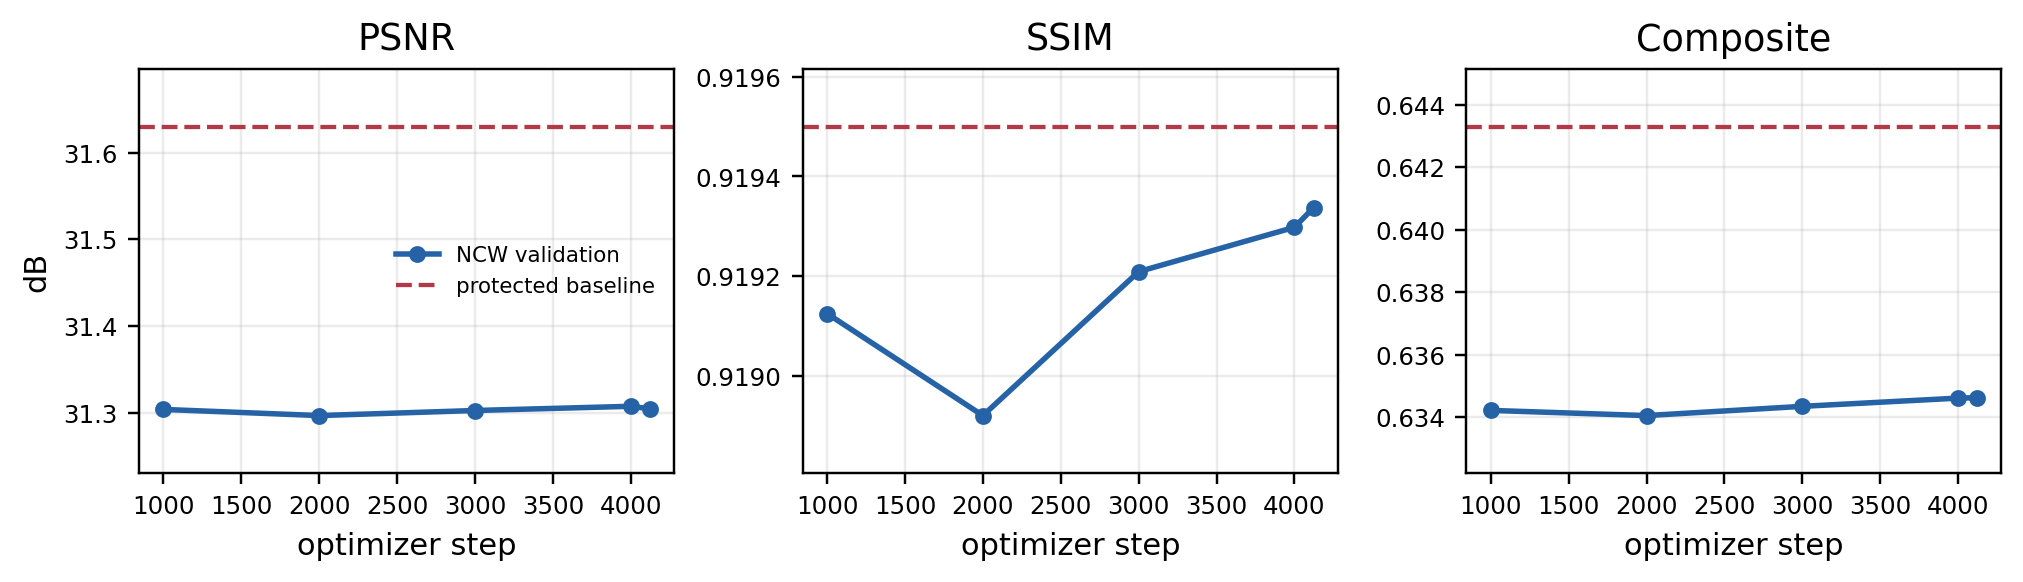
\includegraphics[width=\textwidth]{figs/validation_trajectory.png}
\caption{Validation PSNR, SSIM and composite. Dashed lines show the protected baseline. Phase C gives a small improvement but does not close the baseline gap.}
\end{figure}

The distinction between the best-PSNR and best-composite checkpoints is small but real: step 4122 trades 0.0029 dB for a $3.9\times10^{-5}$ SSIM gain, producing the highest composite of the run.

\section{Interpretation and model-selection decision}
The run is stable but essentially plateaued. Composite varies by only 0.00057 from the worst to best epoch, while every epoch remains about 0.009 below the baseline. Training loss becomes more negative late in phase C, yet the official validation score does not rise proportionally. Additional optimization on the same patch distribution is therefore unlikely to supply the missing 1.7 dB without revisiting the data model, objective calibration, or full-resolution training geometry.

The defensible competition decision is to retain the protected baseline for submission. NCW-NAFNet is preserved as an experimental result because it demonstrates identity-safe conditioning, a complete DirectML-safe training path, and deterministic inference, but it is not claimed as an improvement. The baseline remains better in PSNR, SSIM, and the official composite.

\begin{figure}[h]
\centering
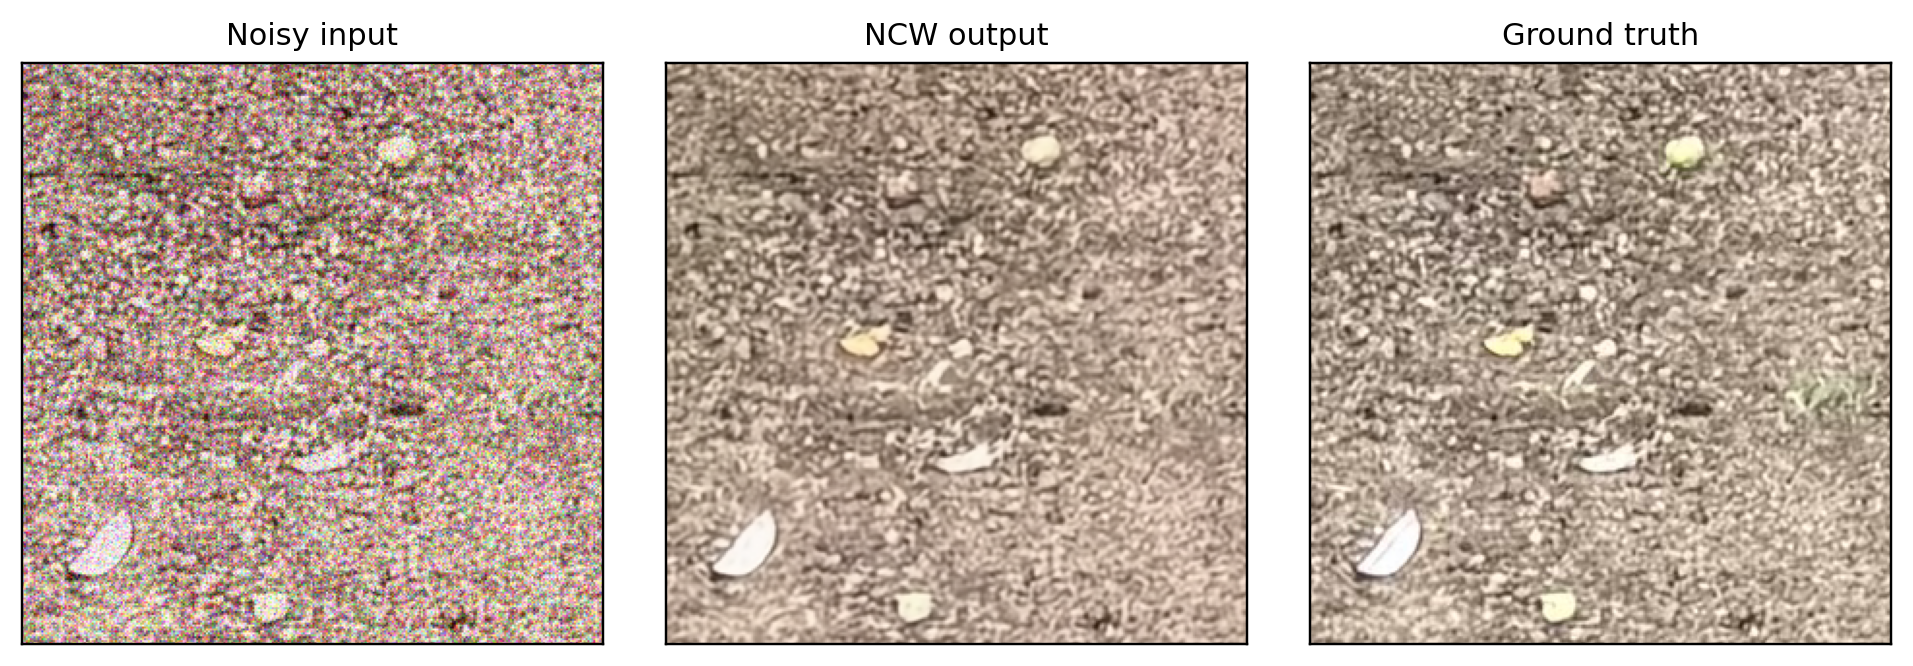
\includegraphics[width=\textwidth]{figs/qualitative_183.png}
\caption{Centre crops for validation image 183, the most severe held-out image by blind noise estimate ($\hat\sigma=40.66$ in 8-bit units). The NCW model removes strong noise while retaining the original exposure, but fine texture differs from the clean target and the aggregate score remains below the baseline.}
\end{figure}

\section{Reproducibility and delivered model}
Selected checkpoint:
\codepath{experiments/ncw_1hour_33db_v5/checkpoints/ncw_1h_best_composite.pth}
SHA-256:
\codepath{30bbb067337916eaf938e1f3349ea347061f1a44e106ac505407c35eac42035f}

The resolved configuration, training log, validation CSV, and final JSON are stored in the experiment directory. Training is reproduced with:
\codepath{python -m ncw.train_1hour --config experiments/ncw_1hour_33db_v5/configs/ncw_1hour_33db_v5.yaml}

Inference is deterministic and uses no test-specific lookup. The 20 hidden test inputs 461--480 were processed with the best-composite checkpoint using the same 256-pixel tiled path. Their denoised PNG files are stored under:
\codepath{experiments/ncw_1hour_33db_v5/test_461_480/denoised/}
Ground truth for these IDs is unavailable and was not used.

\vspace{0.4em}
{\footnotesize\textbf{Backbone reference:} S. Chen et al., ``Simple Baselines for Image Restoration,'' ECCV 2022. All experiment metrics in this report are read from the repository's final \texttt{metrics.csv} and \texttt{final\_result.json}; no value is extrapolated from training loss.}

\end{document}
